\section{Построение прямой, аппроксимирующей множество точек}\label{line}

\subsection{Постановка задачи}\label{line:task}

Дано множество из $n$ точек в плоскости или пространстве. Необходимо построить прямую, максимально близкую к заданному множетсву. Меру близости выберем равной корню из суммы квадратов расстояний от точек множества до прямой. Соответственно, необходимо подобрать такие коэффициенты прямой, чтобы для данного набора точек мера на данном множестве и прямой с этими коэффициентами была минимальна.

\begin{figure}[h]
	{ \noindent \centering
	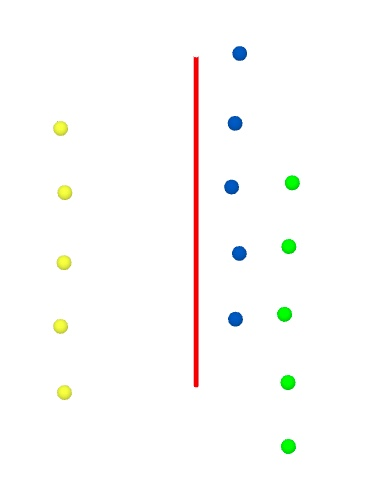
\includegraphics[scale=0.3]{1}
	\caption{Прямая и набор точек в плоскости.}
	}
\end{figure}

\begin{figure}[h]
	{ \noindent \centering
	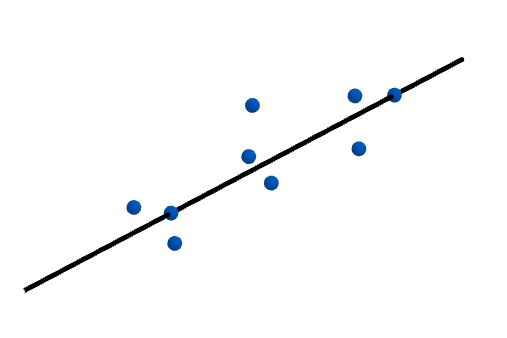
\includegraphics[scale=0.5]{2}
	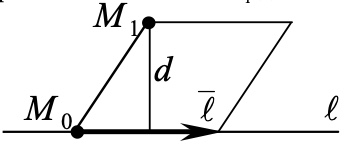
\includegraphics[scale=0.5]{3}
	\caption{Прямая и набор точек в пространстве.}
	}
\end{figure}

\newpage
\subsection{Двумерный случай}\label{line:alg:2dim}

Пусть имеется набор из $n$ точек: $P = \Set{(x_i, y_i)}{i=\ton n}$. 

Будем искать прямую в виде $a \cdot x + b \cdot y + d = 0$, где $a, b, d$ - неизвестные коэффициенты.

По определению расстояние от точки $(x_0, y_0)$ до прямой $ax+by+d=0$ определяется по следующей формуле:

$$\rho (ax+by+d=0, (x_0, y_0)) = \frac{|ax_0+by_0+d|}{\sqrt{a^2+b^2}}$$

Тогда наша мера будет иметь вид:

$$\Lambda (ax+by+d=0,P)=\sqrt{\sum_{i=1}^{n} \frac{(ax_i+by_i+d)^2}{a^2+b^2}}$$

Будем искать нормированное уравнение прямой, которое получается из общего уравнения делением всех членов на $\sqrt{a^2+b^2}$: $a^{'}x+b^{'}y+d^{'}=0$. Тогда расстояние от точки $(x_0,y_0)$ до прямой равно абсолютному значению отклонения и вычисляется по формуле: 

$$\rho (a^{'}x+b^{'}y+d^{'}=0, (x_0, y_0)) = |a^{'}x_0+b^{'}y_0+d^{'}|$$

Тогда наша мера будет иметь вид:

$$\Lambda (a^{'}x+b^{'}y+d^{'}=0,P)=\sqrt{\sum_{i=1}^{n} (a^{'}x_i+b^{'}y_i+d^{'})^2},\;(a^{'})^2+(b^{'})^2=1$$

Будем исследовать не саму меру, а подкоренное выражение, и для простоты будем рассматривать коэффициенты без индексов.

Таким образом, задача свелась к поиску минимального значения выражения $\underset{i=1}{\overset{n}{\sum}}(ax_i+by_i+d)^2$ с ограничением $a^2+b^2=1$.

Будем искать коэффициенты методом Лагранжа. Составим функцию Лагранжа:

$$L(a, b, d, \lambda) = \underset{i=1}{\overset{n}{\sum}}(ax_i+by_i+d)^2 - \lambda (a^2+b^2-1)$$.

Составим систему из четырех уравнений, приравняв к нулю частные производные функции Лагранжа $L(a, b, d, \lambda)$ по $a, b, d$ и $\lambda$:

\begin{center}
	$\begin{cases}
		\frac{\partial}{\partial a} (\underset{i=1}{\overset{n}{\sum}}(ax_i+by_i+d)^2 - \lambda (a^2+b^2-1)) = 0 \\
		\frac{\partial}{\partial b} (\underset{i=1}{\overset{n}{\sum}}(ax_i+by_i+d)^2 - \lambda (a^2+b^2-1)) = 0 \\
		\frac{\partial}{\partial d} (\underset{i=1}{\overset{n}{\sum}}(ax_i+by_i+d)^2 - \lambda (a^2+b^2-1)) = 0 \\
		\frac{\partial}{\partial \lambda} (\underset{i=1}{\overset{n}{\sum}}(ax_i+by_i+d)^2 - \lambda (a^2+b^2-1)) = 0
	\end{cases} \; \Leftrightarrow \;$
\end{center}

\begin{center}
	$\; \Leftrightarrow \;\begin{cases}
		\underset{i=1}{\overset{n}{\sum}}x_i(ax_i+by_i+d) - \lambda a = 0 \\
		\underset{i=1}{\overset{n}{\sum}}y_i(ax_i+by_i+d) - \lambda b = 0 \\
		\underset{i=1}{\overset{n}{\sum}}(ax_i+by_i+d) = 0 \\
		a^2+b^2 = 1
	\end{cases}$
\end{center}

Выразим из третьего уравнения $d$:

$$d = \left(-\frac{\underset{i=1}{\overset{n}{\sum}} x_i}{n}\right) \cdot a + \left(-\frac{\underset{i=1}{\overset{n}{\sum}} y_i}{n}\right) \cdot b$$

Подставим полученное выражение в первые два уравнения:

\begin{center}
	$\begin{cases}
		\underset{i=1}{\overset{n}{\sum}}\left((x_i^2-x_i \cdot\frac{\underset{i=1}{\overset{n}{\sum}} x_i}{n})\cdot a + (x_i y_i - x_i \cdot\frac{\underset{i=1}{\overset{n}{\sum}} y_i}{n})\cdot b\right) - \lambda a = 0\\
		\underset{i=1}{\overset{n}{\sum}}\left((x_i y_i - y_i \cdot\frac{\underset{i=1}{\overset{n}{\sum}} x_i}{n})\cdot a + (y_i^2 - y_i \cdot\frac{\underset{i=1}{\overset{n}{\sum}} y_i}{n})\cdot b\right) - \lambda b = 0\\
	\end{cases}\; \Leftrightarrow \; $
\end{center}

\begin{center}
	$\; \Leftrightarrow \; \begin{pmatrix}
		\underset{i=1}{\overset{n}{\sum}}\left(x_i^2-x_i \cdot\frac{\underset{i=1}{\overset{n}{\sum}} x_i}{n}\right)
		& 
		\underset{i=1}{\overset{n}{\sum}}\left(x_i y_i - x_i \cdot\frac{\underset{i=1}{\overset{n}{\sum}} y_i}{n}\right)
		\\
		\underset{i=1}{\overset{n}{\sum}}\left(x_i y_i - y_i \cdot\frac{\underset{i=1}{\overset{n}{\sum}} x_i}{n}\right)
		&
		\underset{i=1}{\overset{n}{\sum}}\left(y_i^2 - y_i \cdot\frac{\underset{i=1}{\overset{n}{\sum}} y_i}{n}\right)
	\end{pmatrix}\begin{pmatrix}
		a \\ b
	\end{pmatrix} = \lambda \begin{pmatrix}
		a \\ b
	\end{pmatrix}$
\end{center}

\newpage
Таким образом, задача свелась к поиску собственных значений матрицы $A$:

\begin{center}
	$A = \begin{pmatrix}
		\underset{i=1}{\overset{n}{\sum}}x_i^2-\frac{1}{n}\underset{i=1}{(\overset{n}{\sum}} x_i)^2
		& 
		\underset{i=1}{\overset{n}{\sum}}x_i y_i - \frac{1}{n}\underset{i=1}{\overset{n}{\sum}}x_i \underset{i=1}{\overset{n}{\sum}} y_i
		\\
		\underset{i=1}{\overset{n}{\sum}}x_i y_i - \frac{1}{n}\underset{i=1}{\overset{n}{\sum}}x_i \underset{i=1}{\overset{n}{\sum}} y_i
		&
		\underset{i=1}{\overset{n}{\sum}}y_i^2-\frac{1}{n}\underset{i=1}{(\overset{n}{\sum}} y_i)^2
	\end{pmatrix}$
\end{center}

Тем или иным способом, найдем собственные значения. В программе удобно пользоваться методом Якоби, здесь будет изложен прямой метод нахождения собственных значений через характеристический многочлен.

\vspace{0.5cm}
Введем следующие обозначения:

\begin{center}
	$\begin{cases}
		A_{1,1} = \underset{i=1}{\overset{n}{\sum}}x_i^2-\frac{1}{n}\underset{i=1}{(\overset{n}{\sum}} x_i)^2 
		\\
		A_{1,2} = \underset{i=1}{\overset{n}{\sum}}x_i y_i - \frac{1}{n}\underset{i=1}{\overset{n}{\sum}}x_i \underset{i=1}{\overset{n}{\sum}} y_i
		\\
		A_{2,1} = \underset{i=1}{\overset{n}{\sum}}x_i y_i - \frac{1}{n}\underset{i=1}{\overset{n}{\sum}}x_i \underset{i=1}{\overset{n}{\sum}} y_i
		\\
		A_{2,2} = \underset{i=1}{\overset{n}{\sum}}y_i^2-\frac{1}{n}\underset{i=1}{(\overset{n}{\sum}} y_i)^2
	\end{cases} \; \Rightarrow \; A = \begin{pmatrix}
		A_{1,1} & A_{1,2} \\ A_{2,1} & A_{2,2}
	\end{pmatrix}$
\end{center}

Составим характеристическое уравнение:

\begin{center}
	$\begin{vmatrix}
		A_{1,1}-\lambda & A_{1,2} \\ A_{2,1} & A_{2,2}-\lambda
	\end{vmatrix}=0 \; \Rightarrow \; (A_{1,1}-\lambda)(A_{2,2}-\lambda)-A_{1,2} A_{2,1} = 0 \; \Rightarrow \; $
\end{center}

\begin{center}
	$\; \Rightarrow \; \lambda^2 - (A_{1,1}+A_{2,2})\lambda + (A_{1,1} A_{2,2} - A_{1,2} A_{2,1}) = 0 \; \Rightarrow \;$
\end{center}

\begin{center}
	$\; \Rightarrow \; D = (A_{1,1}+A_{2,2})^2-4 (A_{1,1} A_{2,2} - A_{1,2} A_{2,1})$
\end{center}

Будем считать, что в случае решения задачи имеем дело с невырожденным случаем, то $D>0$, тогда:

$$\lambda_1 = \frac{A_{1,1}+A_{2,2} + \sqrt{(A_{1,1}+A_{2,2})^2-4 (A_{1,1} A_{2,2} - A_{1,2} A_{2,1})}}{2}$$

$$\lambda_2 = \frac{A_{1,1}+A_{2,2} - \sqrt{(A_{1,1}+A_{2,2})^2-4 (A_{1,1} A_{2,2} - A_{1,2} A_{2,1})}}{2}$$

\newpage
Получаем две системы:

\begin{center}
	$\begin{cases}
		(A_{1,1} - \lambda_i) a + A_{1,2} b = 0 \\
		A_{2,1} a + (A_{2,2} - \lambda_i) b = 0
	\end{cases},\;i=1,2.$
\end{center}

Данная система однородная, поэтому имеет бесконечное число решений.

Найдем теперь собтвенные векторы. Выразим $a$ через $b$, например, из первых уравнений последних систем:

\begin{center}
	$a = -\frac{A_{1,2}}{A_{1,1}-\lambda_i}b,\;i=1,2$
\end{center}

Положим $b = 1$, тогда $a_i = -\frac{A_{1,2}}{A_{1,1}-\lambda_i},\;i=1,2$.

Уравнение для $d$ через $a$ и $b$ получаем следующее:

\begin{center}
	$d_i = \frac{1}{n}(a_i * \underset{j=1}{\overset{n}{\sum}}x_j + \underset{j=1}{\overset{n}{\sum}}y_j),\;i=1,2$
\end{center}

Далее узнаем значение нашего функционала при данных значениях $a_i, b_i, d$:

\begin{center}
	$L_i (a_i, b = 1, d_i)= \underset{j=1}{\overset{n}{\sum}}(a_i x_j+ y_j + d_i)^2,\;i=1,2$
\end{center}

Выбираем $L = min \{L_1, L_2\}$. Без ограничения общности пусть $L_1 < L_2 \; \Rightarrow \; a = a_1, b = 1, d = d_1$.

Таким образом, итоговые формулы для коэффициентов прмяой получаются следующие:

\begin{center}
	$a = -\frac{A_{1,2}}{A_{1,1}-\lambda_1}, \; b =1, \; d = -\frac{1}{n}(a * \underset{j=1}{\overset{n}{\sum}}x_j + \underset{j=1}{\overset{n}{\sum}}y_j)$
\end{center}.

\newpage
\subsection{Трехмерный случай}\label{line:alg:3dim}

Пусть имеется набор из $n$ точек: $P = \Set{(x_i, y_i, z_i)}{i=\ton n}$. 

Будем искать прямую в параметрическом виде. Пусть $(m, n, p)$ - напрявляющий вектор прямой, $(x_0, y_0, z_0)$ - некоторая точка прямой. Тогда следующая система задает прямую в $\mathbb{R}^3$: 

\begin{center}
	$\mathit{l}: \; \begin{cases}
		x = x_0 + m \cdot t \\
		y = y_0 + n \cdot t \\
		z = z_0 + p \cdot t
	\end{cases}$, где $t \in \mathbb{R}$ - параметр. 
\end{center}

В качестве точки $(x_0, y_0, z_0)$ выбирем центр масс системы данных точек. Таким образом:
$x_0 = \frac{1}{n}\underset{i=1}{\overset{n}{\sum}} x_i, \; y_0 = \frac{1}{n}\underset{i=1}{\overset{n}{\sum}} y_i, \; z_0 = \frac{1}{n}\underset{i=1}{\overset{n}{\sum}} z_i$.

По определению расстояние от точки $M_1$ до прямой $\mathit{l}$ определяется по следующей формуле:

$M_0 (x_0, y_0, z_0)$ - точка на прямой $\mathit{l}$

$\mathit{l} = (m, n, p)$ - напрявляющий вектор прямой

\begin{center}
	$d (M_1, \mathit{l}) = \frac{|[\overline{\mathit{l}}, \overline{M_0 M_1}]|}{|\overline{\mathit{l}}|}$
\end{center}

\begin{center}
	\begin{figure}[h]
	{ 	
		\noindent 
		\centering
		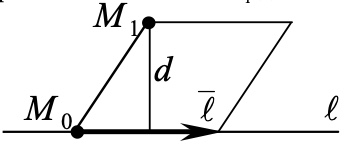
\includegraphics[scale=0.8]{4}
		\caption{Расстояние от точки до прямой.}
	}
\end{figure}
\end{center}

Распишем составляющие элементы формулы для расстояния:

$$|\overline{l}| = \sqrt{m^2 + n^2 + p^2}$$

$$\overline{M_0 M_1} = (x_1 - x_0, y_1 - y_0, z_1 - z_0)$$

$$[\overline{\mathit{l}}, \overline{M_0 M_1}] = \begin{vmatrix}
	\mathbf{i} & \mathbf{j} & \mathbf{k} \\
	m & n & p \\
	x_1 - x_0 & y_1 - y_0 & z_1 - z_0
\end{vmatrix} = $$

$$=\left(\begin{vmatrix}
	n & p \\
	y_1 - y_0 & z_1 - z_0
\end{vmatrix}, -\begin{vmatrix}
	m & p \\
	x_1 - x_0 & z_1 - z_0
\end{vmatrix}, \begin{vmatrix}
	m & n \\
	x_1 - x_0 & y_1 - y_0
\end{vmatrix}\right) = $$

$$= (n (z_1 - z_0) - p (y_1 - y_0), p (x_1 - x_0) - m (z_1 - z_0), m (y_1 - y_0) - n (x_1 - x_0)) = $$

$$ = (n \triangle_{z_1} - p \triangle_{y_1}, p \triangle_{x_1} - m \triangle_{z_1}, m \triangle_{y_1} - n \triangle_{x_1})\text{, где }\begin{cases}
	\triangle_{x_1} = x_1 - x_0 \\
	\triangle_{y_1} = y_1 - y_0 \\
	\triangle_{z_1} = z_1 - z_0
\end{cases}$$

$$|[\overline{\mathit{l}}, \overline{M_0 M_1}]| = \sqrt{(n \triangle_{z_1} - p \triangle_{y_1})^2 + (p \triangle_{x_1} - m \triangle_{z_1})^2 + (m \triangle_{y_1} - n \triangle_{x_1})^2}$$

Тогда формула расстояния принимает вид:

$$d (M_1, \mathit{l}) = \sqrt{\frac{(n \triangle_{z_1} - p \triangle_{y_1})^2 + (p \triangle_{x_1} - m \triangle_{z_1})^2 + (m \triangle_{y_1} - n \triangle_{x_1})^2}{m^2 + n^2 + p^2}}$$

Тогда наша мера примет вид:

$$\Lambda (\mathit{l}, P) = \sqrt{\underset{i=1}{\overset{n}{\sum}} \frac{(n \triangle_{z_i} - p \triangle_{y_i})^2 + (p \triangle_{x_i} - m \triangle_{z_i})^2 + (m \triangle_{y_i} - n \triangle_{x_i})^2}{m^2 + n^2 + p^2} } = $$

$$ = \frac{1}{\sqrt{m^2 + n^2 + p^2}} \sqrt{\underset{i=1}{\overset{n}{\sum}} \left( (n \triangle_{z_i} - p \triangle_{y_i})^2 + (p \triangle_{x_i} - m \triangle_{z_i})^2 + (m \triangle_{y_i} - n \triangle_{x_i})^2 \right)}$$

Будем искать нормированное уравнение прямой, которое получается из общего уравнения делением всех членов на $\sqrt{m^2 + n^2 + p^2}$. Тогда расстояние от точки $(x_0,y_0,z_0)$ до прямой равно абсолютному значению векторного произведения и вычисляется по формуле: 

$$d (M_1, \mathit{l}) = \sqrt{(n \triangle_{z_1} - p \triangle_{y_1})^2 + (p \triangle_{x_1} - m \triangle_{z_1})^2 + (m \triangle_{y_1} - n \triangle_{x_1})^2}$$

Тогда наша мера будет иметь вид:

$$\Lambda (\mathit{l}, P) = \sqrt{\underset{i=1}{\overset{n}{\sum}} \left((n \triangle_{z_i} - p \triangle_{y_i})^2 + (p \triangle_{x_i} - m \triangle_{z_i})^2 + (m \triangle_{y_i} - n \triangle_{x_i})^2 \right)}$$

Будем исследовать не саму меру, а подкоренное выражение.

Таким образом, задача свелась к поиску минимального значения выражения $\underset{i=1}{\overset{n}{\sum}} \left((n \triangle_{z_i} - p \triangle_{y_i})^2 + (p \triangle_{x_i} - m \triangle_{z_i})^2 + (m \triangle_{y_i} - n \triangle_{x_i})^2 \right)$ с ограничением $m^2 + n^2 + p^2=1$.

Будем искать коэффициенты методом Лагранжа. Составим функцию Лагранжа:

$$L(m, n, p, \lambda) = \underset{i=1}{\overset{n}{\sum}} \left((n \triangle_{z_i} - p \triangle_{y_i})^2 + (p \triangle_{x_i} - m \triangle_{z_i})^2 + (m \triangle_{y_i} - n \triangle_{x_i})^2 \right) -$$

$$- \lambda (m^2 + n^2 + p^2-1)$$

Преобразуем выражение под знаком суммы:

$$(n \triangle_{z_i} - p \triangle_{y_i})^2 + (p \triangle_{x_i} - m \triangle_{z_i})^2 + (m \triangle_{y_i} - n \triangle_{x_i})^2 = $$

$$ = n^2 ((\triangle_{x_i})^2 + (\triangle_{z_i})^2) + m^2 ((\triangle_{y_i})^2 + (\triangle_{z_i})^2) + p^2 ((\triangle_{x_i})^2 + (\triangle_{y_i})^2) - $$

$$ - 2 n p \triangle_{y_i} \triangle_{z_i} - 2 m p \triangle_{x_i} \triangle_{z_i} - 2 m n \triangle_{x_i} \triangle_{y_i}$$

Тогда получаем:

$$\underset{i=1}{\overset{n}{\sum}} \left((n \triangle_{z_i} - p \triangle_{y_i})^2 + (p \triangle_{x_i} - m \triangle_{z_i})^2 + (m \triangle_{y_i} - n \triangle_{x_i})^2 \right) = $$

$$ = \underset{i=1}{\overset{n}{\sum}} \Bigl( n^2 ((\triangle_{x_i})^2 + (\triangle_{z_i})^2) + m^2 ((\triangle_{y_i})^2 + (\triangle_{z_i})^2) + p^2 ((\triangle_{x_i})^2 + (\triangle_{y_i})^2) - $$

$$ - 2 n p \triangle_{y_i} \triangle_{z_i} - 2 m p \triangle_{x_i} \triangle_{z_i} - 2 m n \triangle_{x_i} \triangle_{y_i} \Bigl) = $$

$$ = n^2 \underset{i=1}{\overset{n}{\sum}} \left((\triangle_{x_i})^2 + (\triangle_{z_i})^2\right) + m^2 \underset{i=1}{\overset{n}{\sum}} \left((\triangle_{y_i})^2 + (\triangle_{z_i})^2\right) + p^2 \underset{i=1}{\overset{n}{\sum}} \left((\triangle_{x_i})^2 + (\triangle_{y_i})^2\right) - $$

$$ - 2 n p \underset{i=1}{\overset{n}{\sum}} \triangle_{y_i} \triangle_{z_i} - 2 m p \underset{i=1}{\overset{n}{\sum}} \triangle_{x_i} \triangle_{z_i} - 2 m n \underset{i=1}{\overset{n}{\sum}} \triangle_{x_i} \triangle_{y_i}$$

\newpage
Для простоты чтения обозначим коэффициенты в данной формуле следующим образом:

\begin{center}
	$\begin{cases}
		\underset{i=1}{\overset{n}{\sum}} \left((\triangle_{x_i})^2 + (\triangle_{z_i})^2\right) = a_{xz} \\
		\underset{i=1}{\overset{n}{\sum}} \left((\triangle_{y_i})^2 + (\triangle_{z_i})^2\right) = a_{yz} \\
		\underset{i=1}{\overset{n}{\sum}}\left((\triangle_{x_i})^2 + (\triangle_{y_i})^2\right) = a_{xy} \\
		\underset{i=1}{\overset{n}{\sum}} \triangle_{y_i} \triangle_{z_i} = b_{yz} \\
		\underset{i=1}{\overset{n}{\sum}} \triangle_{x_i} \triangle_{z_i} = b_{xz} \\
		\underset{i=1}{\overset{n}{\sum}} \triangle_{x_i} \triangle_{y_i} = b_{xy}
	\end{cases}$
\end{center}

Таким образом, получаем следующую функцию Лагранжа:

$$L(m, n, p, \lambda) = a_{xz} n^2 + a_{yz} m^2 + a_{xy} p^2 - 2 b_{yz} n p - 2 b_{xz} m p  - 2 b_{xy} m n - $$

$$ - \lambda (m^2 + n^2 + p^2-1)$$

Составим систему из четырех уравнений, приравняв к нулю частные производные функции Лагранжа $L(m, n, p, \lambda)$ по $m, n, p$ и $\lambda$:

\begin{center}
	$\begin{cases}
		\frac{\partial}{\partial m} \left(a_{xz} n^2 + a_{yz} m^2 + a_{xy} p^2 - 2 b_{yz} n p - 2 b_{xz} m p  - 2 b_{xy} m n - \lambda (m^2 + n^2 + p^2-1)\right) = 0 \\
		\frac{\partial}{\partial n} \left(a_{xz} n^2 + a_{yz} m^2 + a_{xy} p^2 - 2 b_{yz} n p - 2 b_{xz} m p  - 2 b_{xy} m n - \lambda (m^2 + n^2 + p^2-1)\right) = 0 \\
		\frac{\partial}{\partial p} \left(a_{xz} n^2 + a_{yz} m^2 + a_{xy} p^2 - 2 b_{yz} n p - 2 b_{xz} m p  - 2 b_{xy} m n - \lambda (m^2 + n^2 + p^2-1)\right) = 0 \\
		\frac{\partial}{\partial \lambda} \left(a_{xz} n^2 + a_{yz} m^2 + a_{xy} p^2 - 2 b_{yz} n p - 2 b_{xz} m p  - 2 b_{xy} m n - \lambda (m^2 + n^2 + p^2-1)\right) = 0
	\end{cases} \; \Leftrightarrow \;$
\end{center}

\begin{center}
	$\begin{cases}
		2 a_{yz} m - 2 b_{xz} p - 2 b_{xy} n - 2 \lambda m = 0 \\
		2 a_{xz} n - 2 b_{yz} p - 2 b_{xy} m - 2 \lambda n = 0 \\
		2 a_{xy} p - 2 b_{yz} n - 2 b_{xz} m - 2 \lambda p = 0 \\
		m^2 + n^2 + p^2 = 1
	\end{cases}$
\end{center}

\begin{center}
	$\begin{cases}
		(a_{yz} - \lambda ) m + (-b_{xy}) n + (-b_{xz}) p = 0 \\
		(-b_{xy})m + (a_{xz} - \lambda)n + (-b_{yz})p = 0 \\
		(-b_{xz})m + (-b_{yz})n + (a_{xy} - \lambda)p = 0 \\ 
		m^2 + n^2 + p^2 = 1
	\end{cases}$
\end{center}

Решение первых трех уравнений эквивалентно решению матричного уравнения:

$$\begin{pmatrix}
	a_{yz} - \lambda & -b_{xy} & -b_{xz} \\
	-b_{xy} & a_{xz} - \lambda & -b_{yz} \\
	-b_{xz} & -b_{yz} & a_{xy} - \lambda
\end{pmatrix}\cdot \begin{pmatrix}
	m \\ n \\ p
\end{pmatrix} = 0 \; \Leftrightarrow \; $$

$$\; \Leftrightarrow \; (A - \lambda E)\cdot \begin{pmatrix}
	m \\ n \\ p
\end{pmatrix} = 0,\text{ где } A = \begin{pmatrix}
	a_{yz}  & -b_{xy} & -b_{xz} \\
	-b_{xy} & a_{xz} & -b_{yz} \\
	-b_{xz} & -b_{yz} & a_{xy}
\end{pmatrix}, \; E = \begin{pmatrix}
	1 & 0 & 0 \\
	0 & 1 & 0 \\
	0 & 0 & 1
\end{pmatrix}$$

Тогда задача свелась к поиску собственных значений для матрицы $A$. Тем или иным способом (например, методом Якоби) находим три собственных значения: $\lambda_i,\;i=1,2,3$.

Получаем три системы:

\begin{center}
	$\begin{cases}
		(a_{yz} - \lambda_i ) m + (-b_{xy}) n + (-b_{xz}) p = 0 \\
		(-b_{xy})m + (a_{xz} - \lambda_i)n + (-b_{yz})p = 0 \\
		(-b_{xz})m + (-b_{yz})n + (a_{xy} - \lambda_i)p = 0
	\end{cases}, \; i = 1,2,3$.
\end{center}

Данная система однородная, поэтому имеет бесконечное число решений.

Найдем теперь собтвенные векторы. Выразим $m$ через $n$ и $p$, например, из первых уравнений систем:

$$m = \frac{b_{xy} n + b_{xz} p }{a_{yz} - \lambda_i}, \; i = 1,2,3.$$

Подставим данное выражение во второе и третье уравнения систем:

$$\begin{cases}
	(- \frac{b_{xy}^2}{a_{yz} - \lambda_i} + a_{xz} - \lambda_i) n + (-\frac{b_{xy} b_{xz}}{a_{yz} - \lambda_i} - b_{yz})p = 0 \\
	(-\frac{b_{xz} b_{xy}}{a_{yz} - \lambda_i} - b_{yz}) n + (- \frac{b_{xz}^2}{a_{yz} - \lambda_i} + a_{xy} - \lambda_i) p = 0
\end{cases}, \; i = 1,2,3.$$

Выразим $n$ через $p$ из первого уравнения текущей системы:

$$n = \frac{\frac{b_{xy} b_{xz}}{a_{yz} - \lambda_i} + b_{yz}}{- \frac{b_{xy}^2}{a_{yz} - \lambda_i} + a_{xz} - \lambda_i} p, \; i=1,2,3.$$

Положим $p = 1$. Тогда получаем следующие выражения:

$$n = \frac{\frac{b_{xy} b_{xz}}{a_{yz} - \lambda_i} + b_{yz}}{- \frac{b_{xy}^2}{a_{yz} - \lambda_i} + a_{xz} - \lambda_i}, \; i =1,2,3.$$

$$m = \frac{b_{xy} \left(\frac{\frac{b_{xy} b_{xz}}{a_{yz} - \lambda_i} + b_{yz}}{- \frac{b_{xy}^2}{a_{yz} - \lambda_i} + a_{xz} - \lambda_i}\right) + b_{xz}}{a_{yz} - \lambda_i}, \; i = 1,2,3.$$

Далее узнаем значение нашего функционала при данных значениях $m_i, n_i, p$:

\begin{center}
	$L_i (m_i, n_i, p = 1)= a_{xz} n_i^2 + a_{yz} m_i^2 + a_{xy} - 2 b_{yz} n_i - 2 b_{xz} m_i  - 2 b_{xy} m_i n_i, \;i=1,2,3.$
\end{center}

Выбираем $L = min \{L_1, L_2, L_3\}$. Без ограничения общности пусть $L_1 < L_2 < L_3 \; \Rightarrow \; m = m_1, n = n_1, p = 1$.

Таким образом, итоговые формулы для коэффициентов прмяой получаются следующие:

$$\begin{cases}
	m = \frac{b_{xy} \left(\frac{\frac{b_{xy} b_{xz}}{a_{yz} - \lambda_1} + b_{yz}}{- \frac{b_{xy}^2}{a_{yz} - \lambda_1} + a_{xz} - \lambda_1}\right) + b_{xz}}{a_{yz} - \lambda_1} \\
	n = \frac{\frac{b_{xy} b_{xz}}{a_{yz} - \lambda_1} + b_{yz}}{- \frac{b_{xy}^2}{a_{yz} - \lambda_1} + a_{xz} - \lambda_1} \\
	p = 1 \\
	(x_0, y_0, z_0)\text{ - центр масс системы:} \\
	x_0 = \frac{1}{n}\underset{i=1}{\overset{n}{\sum}} x_i, \; y_0 = \frac{1}{n}\underset{i=1}{\overset{n}{\sum}} y_i, \; z_0 = \frac{1}{n}\underset{i=1}{\overset{n}{\sum}} z_i
\end{cases}$$

\newpage
\subsection{Примеры работы программ}\label{line:application}

\subsubsection{Двумерный случай}\label{line:application:2dim}

\begin{figure}[h]
	{ \noindent \centering
	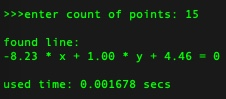
\includegraphics[scale=1]{5}
	\caption{Пример ввода данных и выдачи результата.}
	}
\end{figure}

\begin{figure}[h]
	{ \noindent \centering
	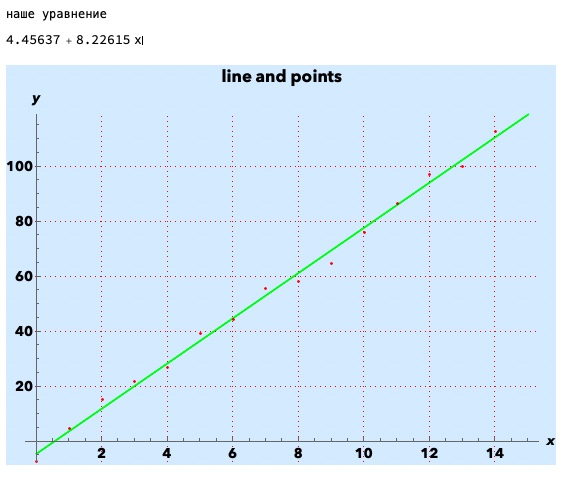
\includegraphics[scale=0.7]{6}
	\caption{Визуализация результата в Wolfram Mathematica.}
	}
\end{figure}

\newpage
\subsubsection{Трехмерный случай}\label{line:application:3dim}

\begin{figure}[h]
	{ \noindent \centering
	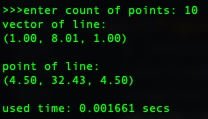
\includegraphics[scale=1]{7}
	\caption{Пример ввода данных и выдачи результата.}
	}
\end{figure}

\begin{figure}[h]
	{ \noindent \centering
	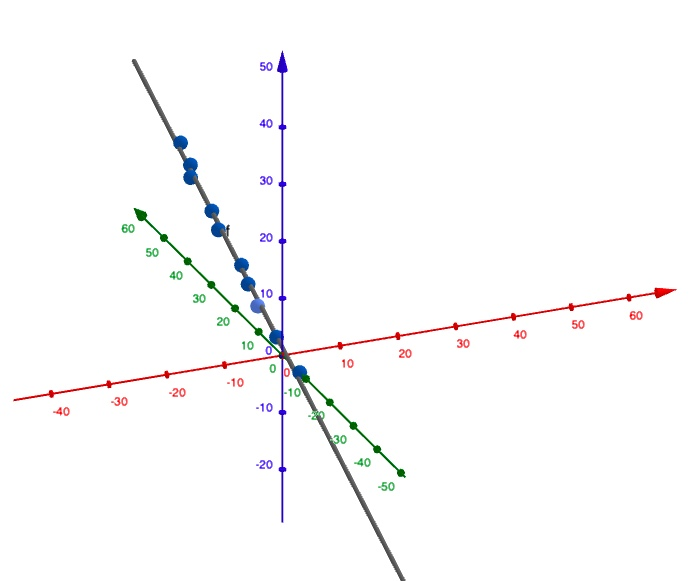
\includegraphics[scale=0.6]{8}
	\caption{Визуализация результата в GeoGebra3D.}
	}
\end{figure}